\documentclass{article}
\usepackage[margin = .7in]{geometry}
\usepackage[dvipdfmx]{graphicx}
\usepackage{listings}
\usepackage{amsmath}
%\usepackage[svgnames]{xcolor}
\usepackage{bm}
\lstset{%
  language={python},
  basicstyle={\small},%
  identifierstyle={\small},%
  commentstyle={\small\itshape},%
  keywordstyle={\small\bfseries},%
  ndkeywordstyle={\small},%
  stringstyle={\small\ttfamily},
  frame={tb},
  breaklines=true,
  columns=[l]{fullflexible},%
  numbers=left,%
  xrightmargin=0zw,%
  xleftmargin=3zw,%
  numberstyle={\scriptsize},%
  stepnumber=1,
  numbersep=1zw,%
  lineskip=-0.5ex%
}


\begin{document}
\title{Macroeconomics 1 2018 S1S2 \\ 
Homework 1}
\author{Kei Ikegami (29186009)}
\maketitle

\section{Problem1}
 We need an additional assumption for stationarity.
 \begin{align}
 	&y_t = c + \phi y_{t-1} + \epsilon_t \nonumber \\
	\Leftrightarrow\ &(1-\phi L)y_t = c + \epsilon_t \nonumber \\
	\Leftrightarrow\ & y_t = (1-\phi L)^{-1} (c + \epsilon_t) = c + \sum_{u = 0}^{\infty} \phi^u L^u \epsilon_t = c + \sum_{u = 0}^{\infty} \phi^u \epsilon_{t-u}
 \end{align}
 For stationarity, it is necessary the above limit exists.  By Chaucy's convergence judgement, we know that it is necessary and sufficient for the convergence of series that the residual, i.e. $\sum_{u = n+1}^{\infty} \phi^u \epsilon_{t-u}$, converges to $0$. Usually, in time series analysis, the Hilbert space, whose product is defined by covariance, is used when the convergence is discussed. Thus if we want to know whether $\sum_{u = n+1}^{\infty} \phi^u \epsilon_{t-u} \to 0$ or not, we must check the convergence w.r.t the norm induced by the covariance product. And for the below calculation we need as assumption that states $Var(y_t) < \infty$. 
\begin{align*}
	\| \sum_{u = n+1}^{\infty} \phi^u \epsilon_{t-u} \| = Var(\sum_{u = n+1}^{\infty} \phi^u \epsilon_{t-u}) = \sum_{n+1}^{\infty} |\phi|^{2u}\sigma^2 = 0
\end{align*}
The second equality is followed by the additional assumption. The third equality is by the assumption $|\phi| < 1$. Now we have the result that $\sum_{u = 0}^{\infty} \phi^u \epsilon_{t-u}$ exists, in other words, the time series is stationary.

Next, I calculate the mean, variance, j-th autocovariance.
\begin{description}
	\item[Mean] By $(1)$, $E[y_t] = E\left[ c + \sum_{u = 0}^{\infty} \phi^u \epsilon_{t-u} \right] = c + 0 = c$
	\item[Variance] By $(1)$, $Var(y_t) = Var\left( \sum_{u = 0}^{\infty} \phi^u \epsilon_{t-u} \right) = \sum_{u=0}^{\infty} |\phi|^{2u} \sigma^2 = \frac{\sigma^2}{1-\phi^2}$
	\item[Autocovariance] $\gamma(t,t-j) = \phi Cov(Y_{t-1}, Y_{t-j}) = \cdots = \phi^j Var(Y_{t-j}) = \frac{\phi^u \sigma^2}{1-\phi^2}$
\end{description}

\section{Problem2}
\subsection{(1)}
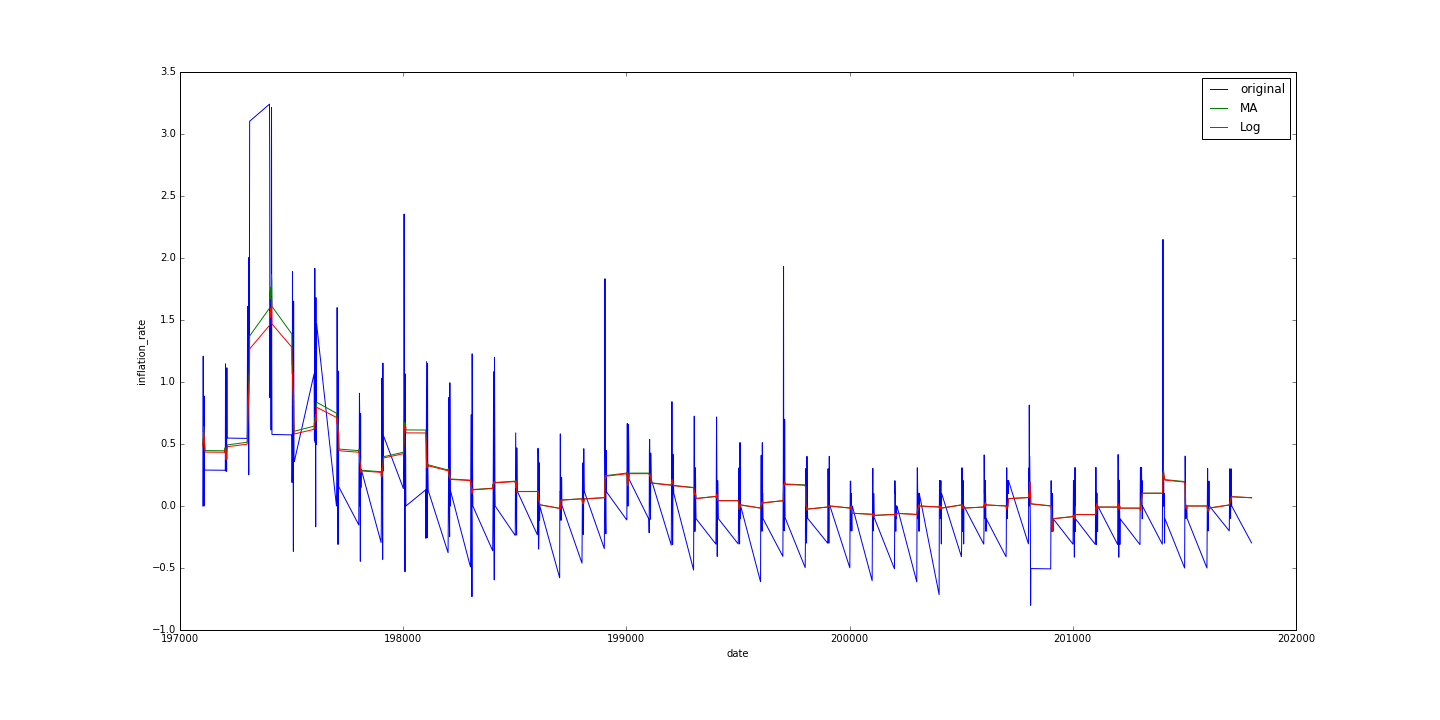
\includegraphics[width = 15cm]{inflation.png}

The Python code is as follows.
\lstinputlisting{hw1-2.py}

\subsection{(3)}
The R code is as follows.
\begin{lstlisting}
# read data
corrected_inflation <- read_csv("~/Desktop/2018summer/macro/hw1/empirics/corrected_inflation.csv")

# time series format
ORI <- ts(corrected_inflation[["original"]])
LOG <- ts(corrected_inflation[["log"]])
MA <- ts(corrected_inflation[["ma"]])

# ma
AIC_ma <- 1:24
for (i in 1:24){
  result <- arima(MA, order = c(i,0,0))
  AIC_ma[i] <- result$aic
}

ma_optimal_p <- which.min(AIC_ma)

# log
AIC_log <- 1:24
for (i in 1:24){
  result <- arima(LOG, order = c(i,0,0))
  AIC_log[i] <- result$aic
}

log_optimal_p <- which.min(AIC_log)
\end{lstlisting}
and $p = 13$ is chosen in both of seasonal adjustments.

\subsection{(3)}
 The estimated coefficients are in the next page. By the table, I see the stochastic significance at $ar1, ar8, ar12$ and $ar13$ in both types of seasonal adjustments. The sign is minus only for $ar12$, and the values are almost the same in the two cases.
 \begin{table}[!htbp] \centering 
  \caption{estimating AR(13)} 
  \label{} 
\begin{tabular}{@{\extracolsep{5pt}}lcc} 
\\[-1.8ex]\hline 
\hline \\[-1.8ex] 
 & \multicolumn{2}{c}{\textit{Dependent variable:}} \\ 
\cline{2-3} 
\\[-1.8ex] & MA & LOG \\ 
\\[-1.8ex] & (1) & (2)\\ 
\hline \\[-1.8ex] 
 ar1 & 1.220$^{***}$ & 1.209$^{***}$ \\ 
  & (0.035) & (0.035) \\ 
  & & \\ 
 ar2 & $-$0.093 & $-$0.078 \\ 
  & (0.057) & (0.056) \\ 
  & & \\ 
 ar3 & $-$0.040 & $-$0.043 \\ 
  & (0.057) & (0.056) \\ 
  & & \\ 
 ar4 & $-$0.079 & $-$0.079 \\ 
  & (0.057) & (0.056) \\ 
  & & \\ 
 ar5 & 0.068 & 0.063 \\ 
  & (0.057) & (0.057) \\ 
  & & \\ 
 ar6 & $-$0.022 & $-$0.021 \\ 
  & (0.057) & (0.057) \\ 
  & & \\ 
 ar7 & $-$0.078 & $-$0.069 \\ 
  & (0.057) & (0.057) \\ 
  & & \\ 
 ar8 & 0.118$^{**}$ & 0.105$^{*}$ \\ 
  & (0.057) & (0.057) \\ 
  & & \\ 
 ar9 & 0.006 & 0.007 \\ 
  & (0.058) & (0.057) \\ 
  & & \\ 
 ar10 & $-$0.011 & $-$0.006 \\ 
  & (0.058) & (0.057) \\ 
  & & \\ 
 ar11 & $-$0.033 & $-$0.028 \\ 
  & (0.058) & (0.057) \\ 
  & & \\ 
 ar12 & $-$0.602$^{***}$ & $-$0.603$^{***}$ \\ 
  & (0.057) & (0.057) \\ 
  & & \\ 
 ar13 & 0.539$^{***}$ & 0.536$^{***}$ \\ 
  & (0.035) & (0.035) \\ 
  & & \\ 
 intercept & 0.211 & 0.203 \\ 
  & (0.150) & (0.143) \\ 
  & & \\ 
\hline \\[-1.8ex] 
Observations & 564 & 564 \\ 
Log Likelihood & 1,214.527 & 1,259.025 \\ 
$\sigma^{2}$ & 0.001 & 0.001 \\ 
Akaike Inf. Crit. & $-$2,399.054 & $-$2,488.050 \\ 
\hline 
\hline \\[-1.8ex] 
\textit{Note:}  & \multicolumn{2}{r}{$^{*}$p$<$0.1; $^{**}$p$<$0.05; $^{***}$p$<$0.01} \\ 
\end{tabular} 
\end{table} 


\section{Problem3}
 I use state-space model for solving this problem. When the first difference series follow AR(2) model, i.e. $\Delta Y_t = \beta_1 \Delta Y_{t-1}+ \beta_2 \Delta Y_{t-2}$, let the state vector and the disturbance vector be
 \begin{align*}
 	X_t = \begin{pmatrix}
	\Delta Y_t \\
	\Delta Y_{t-1}
	\end{pmatrix},\ 
	e_{t} = \begin{pmatrix}
	\epsilon_{t}\\
	0
	\end{pmatrix}
 \end{align*}
 and let the update matrix be
 \begin{align*}
 	F = \begin{pmatrix}
	\beta_1 & \beta_2\\
	1 & 0
	\end{pmatrix}
 \end{align*}
then I have the below description of this model.
\begin{align*}
	X_{t+1} = F X_t + e_{t+1},\ \Delta Y_{t+1} = [1\ 0] X_{t+1}
\end{align*}

 Thus
\begin{align*}
	E_t \left[\Delta Y_{t+j}\right] &= [1\ 0 ]E_t \left[X_{t+j}\right]\\
	&= [1\ 0] E_t \left[ F X_{t+j-1} + e_{t+j} \right]\\
	&= [1\ 0] E_t \left[ F^2 X_{t+j-2} + F e_{t+j-1} + e_{t+j}\right]\\
	&= \cdots\\
	&= [1\ 0] F^j E_t \left[ X_t \right]\\
	&= [1\ 0] F^j \begin{pmatrix} \Delta Y_t\\ \Delta Y_{t-1} \end{pmatrix}
\end{align*}
and then BN trend at $t$, denoted as $\tau_t$, is derived as follows,
\begin{align*}
	\tau_t = y_t + \lim_{J \to \infty} \sum_{j = i}^J E_t\left[ \Delta Y_{t+j} \right] = y_t +  \lim_{J \to \infty} \sum_{j = i}^J [1\ 0] F^j \begin{pmatrix} \Delta Y_t\\ \Delta Y_{t-1} \end{pmatrix} = y_t + [1\ 0] \left( \sum_{j=1}^{\infty} F^j \right) \begin{pmatrix} \Delta Y_t\\ \Delta Y_{t-1} \end{pmatrix}
\end{align*}
I can calculate the limit of series of powered matrices as follows, note that $I$ is the two-dimensional identity matrix,
\begin{align*}
	 \left( \sum_{j=1}^{\infty} F^j \right) = F \left( I - F\right)^{-1} = \frac{1}{1-\beta_1 -\beta_2} \begin{pmatrix} \beta_1 + \beta_2 & \beta_2\\ 1 & \beta_2 \end{pmatrix}
\end{align*}
Then, denoting BN cycle term as $c_t$,  
\begin{align*}
	&\tau_t = y_t + \frac{1}{1-\beta_1 -\beta_2} \left\{ (\beta_1 + \beta_2)\Delta Y_t + \beta_2 \Delta Y_{t-1} \right\}\\
	&c_t = - \frac{1}{1-\beta_1 -\beta_2} \left\{ (\beta_1 + \beta_2)\Delta Y_t + \beta_2 \Delta Y_{t-1} \right\}
\end{align*}


\section{Problem4}

\section{Problem5}
\subsection{(1)}
\begin{align}
	\begin{cases}
	y_t = a_{10} + a_{11}y_{t-1} + a_{12}z_{t-1} + e_{1t}\\
	z_t = a_{20} + a_{21}y_{t-1} + a_{22}z_{t-1} + e_{2t}
	\end{cases}
\end{align}
By $(2)$, I get the below,
\begin{align}
	\begin{cases}
	(1-a_{11}L)y_t = a_{10} + a_{12}z_{t-1} + e_{1t}\\
	(1-a_{22}L)z_t = a_{20} + a_{21}y_{t-1} + e_{2t}
	\end{cases}
	\Rightarrow\ 
	\begin{cases}
	y_t = (1-a_{11}L)^{-1} \left( a_{10} + a_{12}z_{t-1} + e_{1t} \right)\\
	z_t = (1-a_{22}L)^{-1} \left( a_{20} + a_{21}y_{t-1} + e_{2t} \right)
	\end{cases}
\end{align}
Thus I have the following AR(2) form for each time series,
\begin{align}
	\begin{cases}
	y_t = a_{10} + a_{11}y_{t-1} + a_{12} (1-a_{22}L)^{-1} \left( a_{20} + a_{21}y_{t-2} + e_{2t} \right) + e_{1t}\\
	z_t = a_{20} + a_{21} (1-a_{11}L)^{-1} \left( a_{10} + a_{12}z_{t-2} + e_{1t} \right) + a_{22}z_{t-1} + e_{2t}
	\end{cases}
\end{align}

\subsection{(2)}
 Because of symmetry, I show the procedure only for $y_t$ and just show the result w.r.t $z_t$. By $(2),(3)$, I have the following representation.
\begin{align*}
	y_t = &(1-a_{11}L)^{-1}\left\{ a_{10}+(1-a_{22}L)^{-1} a_{12}a_{20} \right\} \\
	+ &a_{12}a_{21}(1-a_{11}L)^{-1}(1-a_{22}L)^{-1}y_{t-2} \\
	+ &a_{12}(1-a_{11}{L})^{-1}(1-a_{22}L)^{-1}e_{2.t-1}\\
	+ &(1-a_{11}L)^{-1}e_{1,t}
\end{align*}
Then I have the following explicit form. Note that $\lambda_1, \lambda_2$ are the inverse of the solutions of $1-(a_{11} + a_{22})x + (a_{11}a_{22} - a_{12}a_{21})x^2$, and I assume that this equation has the real number solution, in other words $(a_{11} +a_{22})^2 -4(a_{11}a_{22} - a_{12}a_{21}) = (a_{11} -aa_{22})^2 + 4a_{12}a_{21} \geq 0$ and $\lambda_1, \lambda_2 < 1$.
\begin{align*}
	y_t = &\left( 1 - a_{12}a_{21} (1-a_{11}L)^{-1}(1-a_{22}L)^{-1} L^2\right)^{-1} \\
	&\left[(1-a_{11}L)^{-1} \left\{ a_{10}+(1-a_{22}L)^{-1} a_{12}a_{20} \right\}
	+ a_{12}(1-a_{11}{L})^{-1}(1-a_{22}L)^{-1}e_{2.t-1} + (1-a_{11}L)^{-1}e_{1,t} \right]\\[8pt]
	= &\left( 1 - \frac{a_{12}a_{21}L^2}{(1-a_{11}L)(1-a_{22}L)}\right)^{-1}\\
	&\left[(1-a_{11}L)^{-1} \left\{ a_{10}+(1-a_{22}L)^{-1} a_{12}a_{20} \right\}
	+ a_{12}(1-a_{11}{L})^{-1}(1-a_{22}L)^{-1}e_{2.t-1} + (1-a_{11}L)^{-1}e_{1,t} \right]\\[8pt]
	=&\left( 1-(a_{11} + a_{22})L + (a_{11}a_{22} - a_{12}a_{21})L^2 \right)^{-1} \left( 1-a_{11}L \right) \left( 1-a_{22}L \right)\\
	&\left[(1-a_{11}L)^{-1} \left\{ a_{10}+(1-a_{22}L)^{-1} a_{12}a_{20} \right\}
	+ a_{12}(1-a_{11}{L})^{-1}(1-a_{22}L)^{-1}e_{2.t-1} + (1-a_{11}L)^{-1}e_{1,t} \right]\\[8pt]
	=& (1- \lambda_1 L)^{-1} (1- \lambda_2 L)^{-1} \left( 1-a_{11}L \right) \left( 1-a_{22}L \right)\\
	&\left[(1-a_{11}L)^{-1} \left\{ a_{10}+(1-a_{22}L)^{-1} a_{12}a_{20} \right\}
	+ a_{12}(1-a_{11}{L})^{-1}(1-a_{22}L)^{-1}e_{2.t-1} + (1-a_{11}L)^{-1}e_{1,t} \right]\\[8pt]
	= & (1- \lambda_1 L)^{-1} (1- \lambda_2 L)^{-1} \left\{ a_{10} - a_{22} a_{10} + a_{12} a_{20} \right\}\\
	&+ a_{12} \left( 1-\lambda_1 L \right)^{-1} (1- \lambda_2 L)^{-1} e_{2,t-1}\\
	&+ (1- \lambda_1 L)^{-1} (1- \lambda_2 L)^{-1} \left( e_{1,t} - a_{22}e_{1,t-1} \right)\\[8pt]
	=&  \left\{ a_{10} - a_{22} a_{10} + a_{12} a_{20} \right\} \left( \sum_{j = 0}^{\infty} \sum_{k = 0}^{j} \lambda_1^k \lambda_2^{j-k} \right)\\
	&+a_{12} \sum_{j = 0}^{\infty}\left( \sum_{k = 0}^j \lambda_1^k \lambda_2^{j-k}\right) e_{2, t-1-j}\\
	&+  \sum_{j = 0}^{\infty} \left( \sum_{k = 0}^j \lambda_1^k \lambda_2^{j-k}\right) e_{1, t-j } - a_{22}  \sum_{j = 0}^{\infty} \left( \sum_{k = 0}^j \lambda_1^k \lambda_2^{j-k}\right) e_{1, t-1-j }
\end{align*}

\subsection{(3)}
 Now I have the explicit representation as follows, since in this case $\lambda_1, \lambda_2 = \frac{3}{5}, 1$.
\begin{align*}
	y_t &= 0.2 \sum_{j = 0}^{\infty} \left( \sum_{k = 0}^{j} \frac{3}{5}^{k} \right) e_{2, t-1-j}+\sum_{j = 0}^{\infty} \left( \sum_{k = 0}^{j} \frac{3}{5}^{k} \right) e_{1, t-j} + 0.8 \sum_{j = 0}^{\infty} \left( \sum_{k = 0}^{j} \frac{3}{5}^{k} \right) e_{1, t-1-j}\\[10pt]
	&= 0.5 \sum_{j = 0}^{\infty} \left( 1 - \frac{3}{5}^j\right) e_{2, t-1-j} + 2.5 \sum_{j = 0}^{\infty} \left( 1 - \frac{3}{5}^j\right) e_{1, t-j} + 2 \sum_{j = 0}^{\infty} \left( 1 - \frac{3}{5}^j\right) e_{1, t-1-j}
\end{align*}
Now each term in the above does not exist, so this is not a stationary process. 

\subsection{(4)}
\begin{align*}
 &\frac{\partial y_{t+s}}{\partial e_{1, t}} = \sum_{k = 0}^{s} \frac{3}{5}^k - 0.8 \sum_{k = 0}^{s-1} \frac{3}{5}^k = \frac{1}{2} + \frac{1}{2} \left( \frac{3}{5} \right)^{s-1}\\[8pt]
 &\frac{\partial y_{t+s}}{\partial e_{2, t}} = 0.2 \sum_{k = 0}^{s-1} \frac{3}{5}^k = \frac{1}{2} -\frac{1}{2} \left( \frac{3}{5}\right)^{s-1}
\end{align*}

\subsection{(5)}
\begin{align*}
	&\frac{\partial y_{t+s}}{\partial \epsilon_{y, t}} = \frac{\partial e_{1,t}}{\partial \epsilon_{y, t}} \frac{\partial y_{t+s}}{\partial e_{1, t}} + \frac{\partial e_{2,t}}{\partial \epsilon_{y, t}} \frac{\partial y_{t+s}}{\partial e_{2, t}} = \frac{\partial y_{t+s}}{\partial e_{1, t}} = \frac{1}{2} + \frac{1}{2} \left( \frac{3}{5} \right)^{s-1}\\[8pt]
	&\frac{\partial y_{t+s}}{\partial \epsilon_{z, t}} = \frac{\partial e_{1,t}}{\partial \epsilon_{z, t}} \frac{\partial y_{t+s}}{\partial e_{1, t}} + \frac{\partial e_{2,t}}{\partial \epsilon_{z, t}} \frac{\partial y_{t+s}}{\partial e_{2, t}} = \frac{1}{2}\left(  \frac{1}{2} + \frac{1}{2} \left( \frac{3}{5} \right)^{s-1}\right) + \frac{1}{2} -\frac{1}{2} \left( \frac{3}{5}\right)^{s-1} = \frac{3}{4} - \frac{1}{4} \left( \frac{3}{5} \right)^{s-1}
\end{align*}

\subsection{(6)}
\begin{align*}
	&\frac{\partial y_{t+s}}{\partial \epsilon_{y, t}} = \frac{\partial e_{1,t}}{\partial \epsilon_{y, t}} \frac{\partial y_{t+s}}{\partial e_{1, t}} + \frac{\partial e_{2,t}}{\partial \epsilon_{y, t}} \frac{\partial y_{t+s}}{\partial e_{2, t}} = \frac{\partial y_{t+s}}{\partial e_{1, t}} + \frac{1}{2} \frac{\partial y_{t+s}}{\partial e_{2, t}}= \frac{1}{2} + \frac{1}{2} \left( \frac{3}{5} \right)^{s-1} + \frac{1}{2} \left( \frac{1}{2} -\frac{1}{2} \left( \frac{3}{5}\right)^{s-1} \right) = \frac{3}{4}+\frac{1}{4}\left( \frac{3}{5} \right)^{s-1} \\[8pt]
	&\frac{\partial y_{t+s}}{\partial \epsilon_{z, t}} = \frac{\partial e_{1,t}}{\partial \epsilon_{z, t}} \frac{\partial y_{t+s}}{\partial e_{1, t}} + \frac{\partial e_{2,t}}{\partial \epsilon_{z, t}} \frac{\partial y_{t+s}}{\partial e_{2, t}} = \frac{1}{2} -\frac{1}{2} \left( \frac{3}{5}\right)^{s-1} 
\end{align*}


\subsection{(7)}

\end{document}
























